
\documentclass[addpoints]{exam}
% Used to insert images
\usepackage[utf8]{inputenc}
\usepackage{graphicx}
\usepackage{color}
\usepackage{tikz}
\usetikzlibrary{shapes.geometric, positioning, arrows.meta}
\usepackage{amsmath} 

\printanswers

\newcommand{\event}{Light}
\def\type{0}

\setlength\fillinlinelength{\textwidth}
\CorrectChoiceEmphasis{\color{red}\bfseries}
\SolutionEmphasis{\color{red}\bfseries}

\setlength\answerclearance{2pt}
\pagestyle{headandfoot}
% Adds a line to the top of the page
\runningheadrule
% The three braces correspond to the different parts of the header: the left is the top left text, middle is top middle, and right is top right.
\runningheader{\event}{\tournament}{\ifnum\type=1 Class Set Test \else Full Name:\hspace{1cm} \fi }
% Adds a line to the bottom of the page
\runningfootrule
% The three braces correspond to the different parts of the footer: the left is the bottom left text, middle is bottom middle, and right is bottom right.
% Doesn't include the title page in the page count 
% \runningfooter{}{Page \the\numexpr\thepage-1\   of \the\numexpr\numpages-1}{}
% Uncomment the line below if you want to include the title page in the page count 
\runningfooter{}{Page \thepage\   of \numpages}{}

\begin{document}
\begin{center}
    {\huge Grade 12 Physics \\ \event
    % Writes key if the answers are shown, otherwise writes test
    \ifprintanswers 
     \space Key
    \else 
     \space \ifnum\type<2 Test \fi \ifnum\type=1 \textbf{(CLASS SET)} \fi \ifnum\type=2 Answer Sheet \fi
    \fi \\ \vspace{3mm}\tournament\vspace{1mm}}
\end{center}
% Change to any picture or just some \vspace{.3\textheight} to leave it blank. [h] ensures that the image is placed in the same place in the document as in the code
\begin{figure}[h]
    \centering
    \includegraphics[height=.3\textheight, width=.6\textwidth, keepaspectratio]{}
\begin{figure}
    \centering
    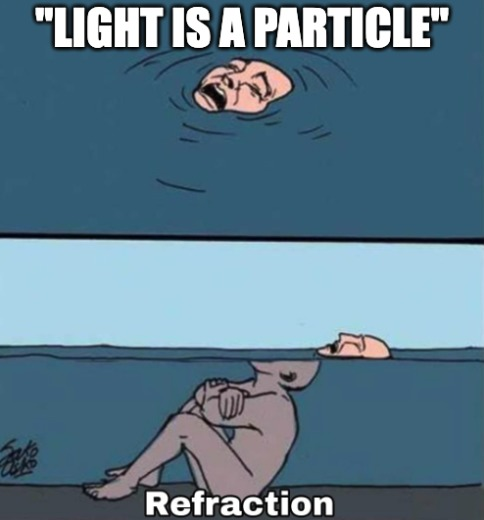
\includegraphics[width=0.5\linewidth]{light-refraction.jpeg}
    \label{fig:enter-label}
\end{figure}
\end{figure}


\begin{center}
    First Name: \ifprintanswers
    \underline{\hspace{3.5cm}}\textbf{KEY}\underline{\hspace{5.5cm}}\\\vspace{5mm}
    \else
        \underline{\hspace{10cm}}\\ \vspace{5mm}
    \fi
    Last Name: \underline{\hspace{10cm}}\\ \vspace{5mm}

\end{center}

% Change the list below to reflect the instructions for your test
\noindent\textbf{\underline{Directions:}}
\begin{itemize}
    % If the test is a class set, an instruction will appear to not write on the test paper.
    \ifnum\type=1 \item \textbf{This test is a class set.} Please do not write any answers on this paper. \fi
    % Adds an instruction 
    \item Please answer to 2 decimal points
    \item The test is designed to be completed in 75 minutes
\end{itemize}
\begin{center}
\textit{For grading use only}\\
% The gradetable has a number of rows that automatically updates. This is not very accurate because of the variance in question size, but it can serve as a starting point. You will probably need to manually update the number of rows of the gradetable (change '\the\numexpr\numpages/13+1' to the desired number of rows).
\multirowgradetable{1}[pages]   
\end{center}

\newpage

\begin{questions}


\section*{Multiple Choice (10 marks)}
\vspace{5mm}

\question[1] Which technology primarily uses total internal reflection?
\begin{choices}
    \correctchoice Fiber optics
    \choice Solar panels
    \choice Microwave ovens
    \choice X-ray machines
\end{choices}

\question[1] What is the wavelength of light with frequency \(6.00 \times 10^{14}\) Hz in a vacuum?
\begin{choices}
    \choice 200 nm
    \correctchoice 500 nm
    \choice 650 nm
    \choice 800 nm
\end{choices}

\question[1] A ray of light passes from water (n = 1.33) into glass (n = 1.50). Which of the following correctly describes how the light ray behaves at the boundary?
\begin{choices}
    \choice It speeds up and bends away from the normal.
    \correctchoice It slows down and bends toward the normal.
    \choice It maintains the same speed but changes direction.
    \choice It slows down and bends away from the normal.
\end{choices}

\question[1] For destructive interference in thin films, the path difference should be:
\begin{choices}
    \choice \(n\lambda\)
    \choice \(2n\lambda\)
    \choice \(\frac{\lambda}{2}\)
    \correctchoice \((n + \frac{1}{2})\lambda\)
\end{choices}

\question[1] Which phenomenon explains rainbow patterns on CDs/DVDs?
\begin{choices}
    \choice Refraction
    \choice Polarization
    \correctchoice Diffraction
    \choice Total internal reflection
\end{choices}

\question[1] A light ray enters glass (n=1.5) from air (n=1.0). If the angle of incidence is 30°, what is the angle of refraction?
\begin{choices}
    \correctchoice 19.47°
    \choice 19.47°
    \choice 30.00°
    \choice 48.59°
\end{choices}

\question[1] A convex lens has a focal length of 15 cm. An object is placed 10 cm from the lens. The image formed will be:
\begin{choices}
    \choice Real, inverted, and larger than the object.
    \correctchoice Virtual, upright, and larger than the object.
    \choice Real, inverted, and smaller than the object.
    \choice Virtual, upright, and smaller than the object.
\end{choices}

\question[1] The energy of a photon with wavelength 450 nm is:
\begin{choices}
    \choice \(1.33 \times 10^{-19}\) J
    \choice \(2.89 \times 10^{-19}\) J
    \choice \(5.67 \times 10^{-19}\) J
    \correctchoice \(4.42 \times 10^{-19}\) J
\end{choices}

\question[1] Polarization by reflection occurs when:
\begin{choices}
    \correctchoice Angle equals Brewster's angle
    \choice Light is completely absorbed
    \choice Total internal reflection occurs
    \choice Light is transmitted
\end{choices}

\question[1] A coil of wire moves through a magnetic field, inducing a current. If the speed of the coil’s motion doubles, the induced current will:
\begin{choices}
    \choice Stay the same
    \choice Stay the same
    \correctchoice Double
    \choice Become zero
\end{choices}

\section*{Long Answer (40 marks)}

\question Thin Film Interference
\begin{parts}
    \part[4] A soap bubble (n=1.33) in air appears yellow-green (λ=550 nm) at its thinnest point. Calculate the minimum thickness of the film.
    \part[4] Explain why thicker regions of the bubble appear redder, and why colors change when viewed from different angles.
\end{parts}
\begin{solution} [8cm]

\textbf{11. Thin Film Interference}  

\textbf{(a) Minimum thickness of the film:}  
For constructive interference in a thin film with a higher refractive index than air, the condition is:  
\[
2 t = \frac{\lambda}{2n}
\]
Solving for \( t \):  
\[
 t = \frac{\lambda}{4n} = \frac{550 \text{ nm}}{4 \times 1.33}
\]
\[
 t = \frac{550}{5.32} = 103.38 \text{ nm}
\]

\textbf{(b) Color changes in different thicknesses and angles:}  
- Thicker regions of the film cause a longer path difference, shifting towards longer wavelengths (redder colors).
- Changing the viewing angle alters the effective thickness and interference conditions, leading to a spectrum of colors.

\end{solution}


\question Double-Slit Interference
\begin{parts}
    \part[4] Calculate fringe spacing for 650 nm light through slits 0.15 mm apart, projected 1.2 m away
    \part[4] Explain what happens to the pattern if blue light (λ=470 nm) replaces red light (λ=700 nm)
\end{parts}
\begin{solution} [8cm]

\textbf{12. Double-Slit Interference}  

\textbf{(a) Fringe spacing:}  
The fringe spacing is given by:  
\[
 y = \frac{\lambda L}{d}
\]
Substituting the values:  
\[
 y = \frac{(650 \times 10^{-9} \text{ m}) (1.2 \text{ m})}{0.15 \times 10^{-3} \text{ m}}
\]
\[
 y = \frac{7.8 \times 10^{-4}}{1.5 \times 10^{-4}} = 5.2 \text{ mm}
\]

\textbf{(b) Effect of replacing red light with blue light:}  
- Blue light has a shorter wavelength than red light.
- Since \( y \propto \lambda \), the fringe spacing decreases, making the fringes closer together.


\end{solution}




\question Layered Media Refraction
\begin{parts}
    \part[4] Light travels from air (n=1.00) through 5 cm of water (n=1.33), then 3 cm of glass (n=1.52). If the initial angle is 30°, calculate the final angle in the glass.
    \part[4] Calculate the total lateral displacement of the light beam through the system.
\end{parts}
\begin{solution} [8cm]

\textbf{(a) Final angle in the glass:}  

Using Snell’s law:  
\[
n_1 \sin \theta_1 = n_2 \sin \theta_2
\]
For air to water (\( n_1 = 1.00 \), \( n_2 = 1.33 \), \( \theta_1 = 30^\circ \)):  
\[
1.00 \sin 30^\circ = 1.33 \sin \theta_2
\]
\[
0.500 = 1.33 \sin \theta_2
\]
\[
\sin \theta_2 = \frac{0.500}{1.33} = 0.3759
\]
\[
\theta_2 = \sin^{-1}(0.3759) = 22.1^\circ
\]

For water to glass (\( n_2 = 1.33 \), \( n_3 = 1.52 \)):  
\[
1.33 \sin 22.1^\circ = 1.52 \sin \theta_3
\]
\[
1.33 \times 0.3759 = 1.52 \sin \theta_3
\]
\[
0.500 = 1.52 \sin \theta_3
\]
\[
\sin \theta_3 = \frac{0.500}{1.52} = 0.3289
\]
\[
\theta_3 = \sin^{-1}(0.3289) = 19.2^\circ
\]

\textbf{(b) Total lateral displacement:}  

Lateral displacement in each medium:  
\[
d = t \tan \theta
\]
For water (\( t_1 = 5 \) cm, \( \theta_2 = 22.1^\circ \)):  
\[
d_1 = 5 \tan 22.1^\circ = 5 \times 0.406 = 2.03 \text{ cm}
\]
For glass (\( t_2 = 3 \) cm, \( \theta_3 = 19.2^\circ \)):  
\[
d_2 = 3 \tan 19.2^\circ = 3 \times 0.348 = 1.04 \text{ cm}
\]
Total lateral displacement:  
\[
d_{\text{total}} = d_1 + d_2 = 2.03 + 1.04 = 3.07 \text{ cm}
\]
\end{solution}


\end{questions}

\end{document}
